\documentclass[a4paper, 10pt]{article}

\usepackage[T1]{fontenc}
\usepackage[portuguese]{babel}
\usepackage[utf8]{inputenc}
\inputencoding{utf8}
\usepackage{array}
\usepackage{graphicx}
\usepackage{caption}
\usepackage{subcaption}
\usepackage{amsmath}
\usepackage{float}
\usepackage{placeins}
\usepackage{amsfonts}
\usepackage{amssymb}
\usepackage{listings}
\usepackage{xcolor}

\definecolor{dkgreen}{rgb}{0,0.6,0}
\definecolor{gray}{rgb}{0.5,0.5,0.5}
\definecolor{mauve}{rgb}{0.58,0,0.82}
\definecolor{blue}{rgb}{0.75,0.75,0.95}
\definecolor{red}{rgb}{1.0,0.0,0.0}

\restylefloat{figure}

\usepackage{verbatim}
\usepackage{framed}
\usepackage{indentfirst}

\title{Trabalho 1 \\Aprendizado de Máquina - 2018.1\\ Universidade Federal do Rio de Janeiro
}

\author{Raphael Barros Parreira \\
}

\date{20 de Julho de 2018}
\begin{document}

\maketitle
\thispagestyle{empty}
\begin{figure}[H]
	\centering
	
\includegraphics[keepaspectratio,width=0.8\textwidth]{img/minerva}
\end{figure}


\newpage
\renewcommand*\contentsname{Índice}
\tableofcontents
\newpage


\section{Introdução}

O trabalho consiste na participação de uma competição do Kaggle. A competição prevê a predição de preços de casas baseada em suas características. Para isso, é necessário que seja aplicado o conhecimento adquirido no curso para fazer com que um programa de computador seja capaz de aprender como fazer essa predição baseado numa base de dados conhecida previamente.

Além de fornecer a base de dados de treino (que contém os preços das casas) e a base de teste (base usada para fazer a predição final), o Kaggle também fornece materiais de outros participantes, que auxiliam o processo de aprendizagem e desenvolvimento do programa.

Uma outra informação presente na competição é a descrição de cada uma das características possíveis das casas, para que auxilie o desenvolvedor a escolher o que fazer com cada uma das colunas da base de dados.

\subsection{Arquivos fornecidos pelo Kaggle}

\begin{itemize}
\item \textbf{$train.csv$} - dataset de treino
\item \textbf{$test.csv$} - dataset de teste
\item \textbf{$data_description.txt$} - descrição de cada uma das características da casa
\item \textbf{$sample_submission.csv$} - exemplo de arquivo para ser submetido ao Kaggle
\end{itemize}

\subsection{Como funciona a submissão à competição}

Para submeter a reposta ao Kaggle, o competidor deve criar um arquivo $ .csv $ (valores separados por vírgulas) contendo duas colunas: Id e SalePrice. Além disso, os preços e os Ids devem corresponder, para que o sistema do Kaggle consiga validar o preço para o seu respectivo Id.

Ao enviar o arquivo para a validação, o Kaggle verifica a pontuação da tentativa e informa a colocação.

\subsection{Premissas}

O trabalho apresenta, como premissa, o fato de se usar apenas algoritmos de regressão para realizar a predição dos preços. Além disso, deixou livre a escolha dos algoritmos por parte do participante. Sendo assim, os algoritmos escolhidos foram: Ridge, Lasso, ElasticNet e KernelRidge.

\clearpage
\section{Pré-processamento dos dados}

Para que os algoritmos tenham uma maior eficácia, é necessário que os dados fornecidos pelo desafio sejam processados. Esse processamento é responsável por excluir dados que prejudiquem o aprendizado, preencher os faltantes (quando possível), criação de novas colunas, compilando e/ou combinando as características já existentes e, se necessário, manipulação dos dados para simplificação de categorias, com o objetivo de tornar o conjunto de dados mais enxuto.

\subsection{Tratamento de Outliers}

Um dos passos importantes para o tratamento de dados, é a identificação e remoção de pontos muito fora do padrão, para que o algortimo não se atrapalhe com pontos que não fazem parte do conjunto de dados normalmente, que tem pouca ocorrência.

No caso desse desafio, o próprio autor do dataset indica que existem outliers no conjunto de dados de treino.

Podemos observar os outliers no gráfico abaixo.

\lstset {
  backgroundcolor=\color{white}, 
   basicstyle=\tiny,       
  breakatwhitespace=false,
  breaklines=true,
  captionpos=b,
   commentstyle=\color{red},
   frame=single,
   keepspaces=true,
   language=Python,
   numbers=left,
   numbersep=5pt,
   numberstyle=\tiny\color{gray},
   showspaces=false,
   showstringspaces=false,
   showtabs=false,
   stepnumber=1,
   stringstyle=\color{mauve},
   tabsize=1,
}
\begin{lstlisting}
import matplotlib.pyplot as plt 
import pandas as pd

df_train=pd.read_csv('./input/train.csv')

fig, ax = plt.subplots()
ax.scatter(x = df_train['GrLivArea'], y = df_train['SalePrice'])
plt.ylabel('SalePrice', fontsize=13)
plt.xlabel('GrLivArea', fontsize=13)
plt.show()

\end{lstlisting}

\begin{figure}[H]
	\centering
	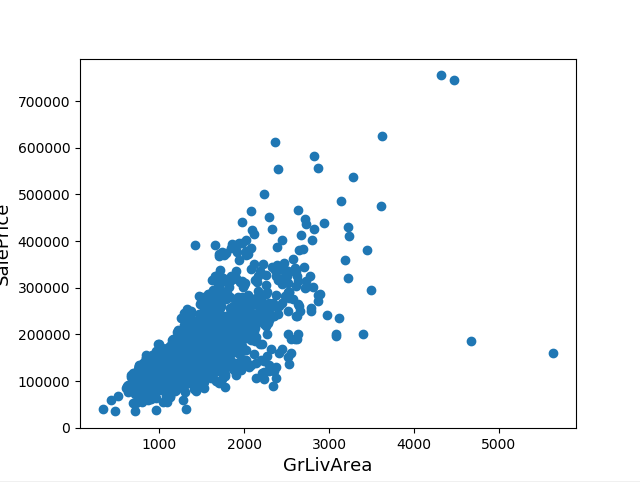
\includegraphics[keepaspectratio,width=1\textwidth]{img/outlier.png}
\end{figure}

O autor recomenda remover os dois pontos que tem uma grande área, e que foram vendidos por um preço muito baixo. Que são os dois pontos com $ GrLivArea > 4.000 $ \& $ SalePrice < 300.000 $.

\lstset {
  backgroundcolor=\color{white}, 
   basicstyle=\tiny,       
  breakatwhitespace=false,
  breaklines=true,
  captionpos=b,
   commentstyle=\color{red},
   frame=single,
   keepspaces=true,
   language=Python,
   numbers=left,
   numbersep=5pt,
   numberstyle=\tiny\color{gray},
   showspaces=false,
   showstringspaces=false,
   showtabs=false,
   stepnumber=1,
   stringstyle=\color{mauve},
   tabsize=1,
}
\begin{lstlisting}
df_train = df_train.drop(df_train[(df_train['GrLivArea']>4000) & (df_train['SalePrice']<300000)].index)

fig, ax = plt.subplots()
ax.scatter(x = df_train['GrLivArea'], y = df_train['SalePrice'])
plt.ylabel('SalePrice', fontsize=13)
plt.xlabel('GrLivArea', fontsize=13)
plt.show()

\end{lstlisting}

\begin{figure}[H]
	\centering
	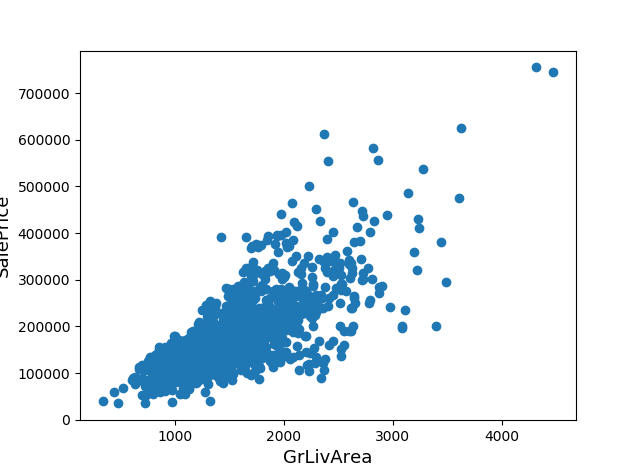
\includegraphics[keepaspectratio,width=1\textwidth]{img/outlier-retirados.png}
\end{figure}

\subsection{Variável Alvo}

Como dito anteriormente, a variável a ser calculada é o preço do imóvel. Sendo assim, é necessário avaliar a relação do SalePrice com as outras variáveis do conjunto de dados, e também a sua normalização.


\lstset {
  backgroundcolor=\color{white}, 
   basicstyle=\tiny,       
  breakatwhitespace=false,
  breaklines=true,
  captionpos=b,
   commentstyle=\color{red},
   frame=single,
   keepspaces=true,
   language=Python,
   numbers=left,
   numbersep=5pt,
   numberstyle=\tiny\color{gray},
   showspaces=false,
   showstringspaces=false,
   showtabs=false,
   stepnumber=1,
   stringstyle=\color{mauve},
   tabsize=1,
}
\begin{lstlisting}
sns.distplot(df_train['SalePrice'] , fit=norm);

# Get the fitted parameters used by the function
(mu, sigma) = norm.fit(df_train['SalePrice'])
print( '\n mu = {:.2f} and sigma = {:.2f}\n'.format(mu, sigma))

#Now plot the distribution
plt.legend(['Normal dist. ($\mu=$ {:.2f} and $\sigma=$ {:.2f} )'.format(mu, sigma)],
            loc='best')
plt.ylabel('Frequency')
plt.title('SalePrice distribution')

#Get also the QQ-plot
fig = plt.figure()
res = stats.probplot(df_train['SalePrice'], plot=plt)
plt.show()

\end{lstlisting}

\begin{figure}[H]
	\centering
	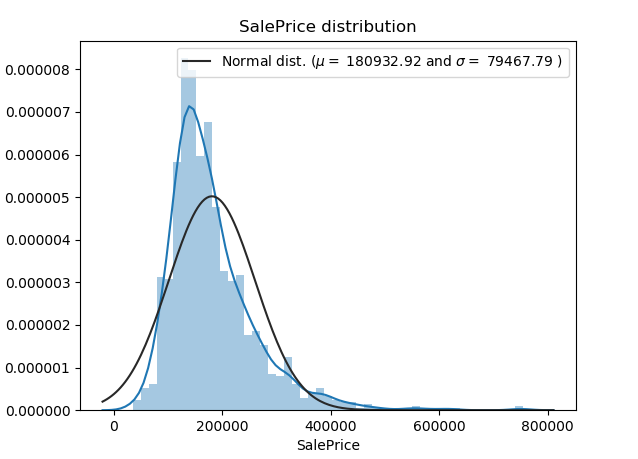
\includegraphics[keepaspectratio,width=1\textwidth]{img/saleprice-normalizado.png}
\end{figure}

\begin{figure}[H]
	\centering
	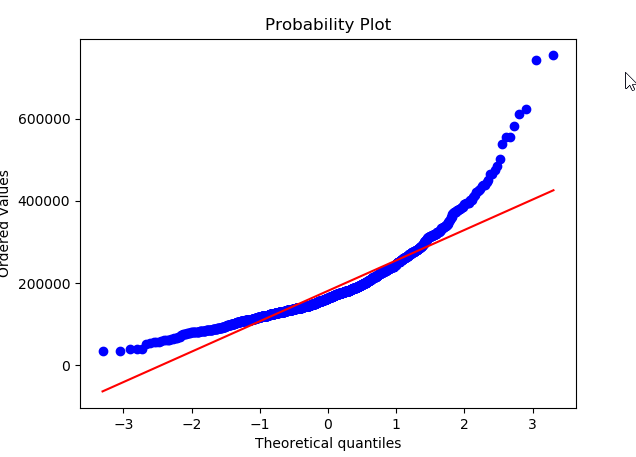
\includegraphics[keepaspectratio,width=1\textwidth]{img/saleprice-prob.png}
\end{figure}

Como podemos perceber, a variável é \textit{skewed} positivamente. Com isso, para que os regressores lineares funcionem de uma melhor forma, é importante que a variável seja normalizada. Mas é importante lembrar que, para submeter a resposta para avaliação, é nessário reverter o log para o preço normal.


\lstset {
  backgroundcolor=\color{white}, 
   basicstyle=\tiny,       
  breakatwhitespace=false,
  breaklines=true,
  captionpos=b,
   commentstyle=\color{red},
   frame=single,
   keepspaces=true,
   language=Python,
   numbers=left,
   numbersep=5pt,
   numberstyle=\tiny\color{gray},
   showspaces=false,
   showstringspaces=false,
   showtabs=false,
   stepnumber=1,
   stringstyle=\color{mauve},
   tabsize=1,
}
\begin{lstlisting}
df_train["SalePrice"] = np.log1p(df_train["SalePrice"])

\end{lstlisting}

\begin{figure}[H]
	\centering
	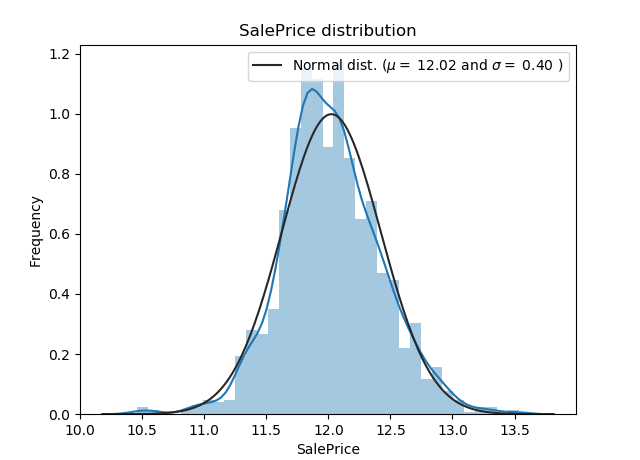
\includegraphics[keepaspectratio,width=1\textwidth]{img/saleprice-norm.png}
\end{figure}

\begin{figure}[H]
	\centering
	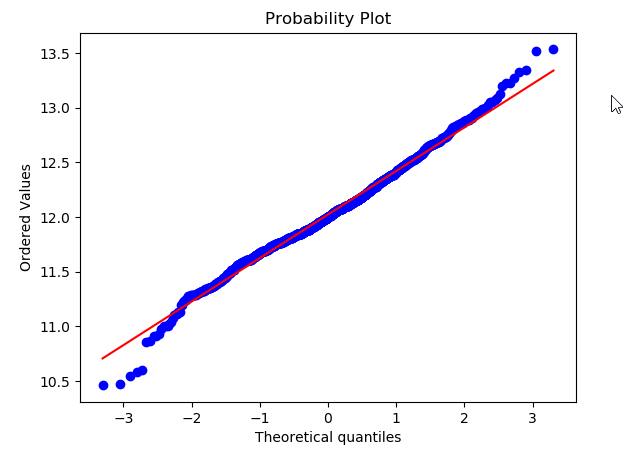
\includegraphics[keepaspectratio,width=1\textwidth]{img/saleprice-prob-norm.png}
\end{figure}

\clearpage
\section{Trechos importantes do código}

Primeiramente é importante ressaltar que os trechos de códigos vistos abaixo foram escritos na linguagem do Matlab.

\subsection{Variáveis importantes}
\lstset {
  backgroundcolor=\color{white}, 
   basicstyle=\tiny,       
  breakatwhitespace=false,
  breaklines=true,
  captionpos=b,
   commentstyle=\color{red},
   frame=single,
   keepspaces=true,
   language=Matlab,
   numbers=left,
   numbersep=5pt,
   numberstyle=\tiny\color{gray},
   showspaces=false,
   showstringspaces=false,
   showtabs=false,
   stepnumber=1,
   stringstyle=\color{mauve},
   tabsize=1,
}
\begin{lstlisting}
handles.ns = 0;
handles.Soriginal = [];

.
.
.

chegada = str2num(get(handles.edit1, 'String'));

tempComp = str2num(get(handles.edit2, 'String'));

deadline = str2num(get(handles.edit3, 'String'));

prioridade = str2num(get(handles.edit4, 'String'));

\end{lstlisting}

No trecho acima pode-se observar algumas variáveis importantes para o bom funcionamento do protocolo estudado, em que:


\begin{itemize}
  \item handles.ns é o número de semáforos utilizados por um determinado conjunto de tarefas;
  \item handles.Soriginal são os parâmetros de cada semáforo e sua relação com cada tarefa, ou seja, quanto tempo a tarefa irá utilizá-lo e apartir de que instante ela necessitará desse semáforo.
\end{itemize}

São as variáveis globais do código, isto é, podem ser acessadas por qualquer função do programa.
Já as  variáveis abaixo, são as variaveis locais da função principal do programa.

\begin{itemize}
  \item chegada é um array que contém os tempo de chegada de cada tarefa;
  \item tempComp é um array que armazena os tempos de execução para cada tarefa;
  \item deadline array para armazenar os tempos limites(deadlines) de cada tarefa a ser executada;
  \item prioridade é um array que armazena as prioridades "normal" de cada tarefa;
\end{itemize}

É importante observar a função $get(handle. , '')$ vistas na atribuição de cada uma dessas últimas variáveis listadas, isso uma vez que esta função é responsável por adquirir o valor do campo correspondente àquela variável na interface.


\subsection{Botão de inserção}

Nesta seção analisa-se o funcionamento do botão \textit{Inserir}. 

\lstset {
  backgroundcolor=\color{white}, 
   basicstyle=\tiny,       
  breakatwhitespace=false,
  breaklines=true,
  captionpos=b,
   commentstyle=\color{red},
   frame=single,
   keepspaces=true,
   language=Matlab,
   numbers=left,
   numbersep=5pt,
   numberstyle=\tiny\color{gray},
   showspaces=false,
   showstringspaces=false,
   showtabs=false,
   stepnumber=1,
   stringstyle=\color{mauve},
   tabsize=1,
}
\begin{lstlisting}
function pushbutton2_Callback(hObject, eventdata, handles)
w = handles.ns + 1;
initial_temp = cellstr(get(handles.listbox1,'String'))
a = get(handles.edit6, 'String');
temp = [initial_temp; a];
set(handles.listbox1, 'String', temp);
b =  str2num(a);
handles.ns = w;
handles.Soriginal(:,:,w) = str2num(get(handles.edit6, 'String'));
guidata(hObject, handles);

\end{lstlisting}

Este botão, como o nome sugere serve para a inserção de um semáforo na execução das tarefas, para isso é necessário que se escreva os parâmetros do semáforo, isto é, tempo em que cada tarefafaz o requerimento para utilizá-lo; duração da execução de cada tarefa utilizando este semáforo e por fim o "status" da tarefa em relação ao semáforo sendo:

\begin{enumerate}
\item 0 $\rightarrow$ para tarefas inativas;
\item 1 $\rightarrow$ para tarefas ativas;
\item 2 $\rightarrow$ para tarefas finalizadas ou inexistentes em relação ao semáforo.
\end{enumerate}

\subsection{Loop principal}

Nesta seção é mostrado o trecho do código onde "a mágica acontece", isso tendo em vista que é nesse trecho que todas as comparações e definições de prioridades ocorrem como pode ser visto abaixo:

\lstset {
   backgroundcolor=\color{white}, 
   basicstyle=\tiny,       
   breakatwhitespace=false,
   breaklines=true,
   captionpos=b,
   commentstyle=\color{red},
   frame=single,
   keepspaces=true,
   language= Matlab,
   numbers=left,
   numbersep=5pt,
   numberstyle=\tiny\color{gray},
   showspaces=false,
   showstringspaces=false,
   showtabs=false,
   stepnumber=1,
   stringstyle=\color{mauve},
   tabsize=1,
}
\begin{lstlisting}
if length(tam)< 3;
    tam(3) = 1;
end
for i=1:tam(3)
    prioridadeBloqueada(i)=101;
    
    [cores(i,1),cores(i,2),cores(i,3)]=HSVtoRGB(1+(i-1)*(358/(tam(3))),.41,.86);
    
    for j=1:tam(1)
        if S(j,2,i)>0
            C(i)=j;
            break;
        end
    end
end

C(length(C)+1)=100;

tempo=0;

for i=1:length(chegada)
    prioridadeAtiva(i)=100;
end


ativos=zeros(length(chegada));


largura=max((sum(sum(S(:,2,:)))+sum(tempComp))*1.2,(max(deadline)+2));


tic;


cla
hold on
grid on
set(gca,'xtick',[0:1:largura])

xlim([0,largura])
ylim([0,20*(1+length(chegada))])
set(gca,'YTick',[0:20:20*length(chegada)])

for i=1:length(chegada)
    plot([chegada(i),chegada(i)],[20*(length(chegada)+1-i),20*(length(chegada)+1-i)+15],'-.b','LineWidth',2)
    plot([deadline(i),deadline(i)],[20*(length(chegada)+1-i),20*(length(chegada)+1-i)+15],'-.r','LineWidth',2)
end

drawnow


SmaiorCeiling=length(C);


while (true)

    paraContador=toc;
      

    tic;
    

    tempo=tempo+paraContador;

    for i=1:length(chegada)
        if ~ativos(i) && chegada(i)<=tempo
            ativos(i)=1;
            prioridadeAtiva(i)=prioridade(i);
        end            
    end
    

    [minimo,proximoProcesso]=min(prioridadeAtiva);
      
    for i=1:tam(3)
        if S(proximoProcesso,3,i)==0 & compFeita(proximoProcesso) >= S(proximoProcesso,1,i)
            for j=1:tam(3)
                if any(S(:,3,j)==1) & C(SmaiorCeiling)>C(j)
                    SmaiorCeiling=j;
                end
            end
            
            if prioridadeAtiva(proximoProcesso)<C(SmaiorCeiling) | any(S(proximoProcesso,3,:)==1)
                S(proximoProcesso,3,i)=1;
                
            else

                prioridadeAtiva(find((S(:,3,SmaiorCeiling))==1))=proximoProcesso-0.1;
                
                prioridadeBloqueada(SmaiorCeiling)=proximoProcesso-0.1;
            end
        end
    end
    
    if minimo<100
        
        if ~(any(S(proximoProcesso,3,:)==1))
        
            compRestante(proximoProcesso)=compRestante(proximoProcesso)-paraContador;
            if compRestante(proximoProcesso)<0
                compRestante(proximoProcesso)=0;
                tempo=tempo+compRestante(proximoProcesso);
                paraContador=paraContador-compRestante(proximoProcesso);
            end
            
            compFeita(proximoProcesso)=compFeita(proximoProcesso)+paraContador;

            rectangle('Position',[tempo-paraContador,20*(length(chegada)+1-proximoProcesso),paraContador,10],'FaceColor',[0.6 0.6 0.9],'LineStyle','None');
            drawnow
            
        else

            zonaAtiva=[0 0];
            for i=1:tam(3)
                if S(proximoProcesso,3,i)==1 & S(proximoProcesso,1,i)>=zonaAtiva(2)
                    zonaAtiva=[i S(proximoProcesso,1,i)];
                end
            end            
            
            S(proximoProcesso,2,zonaAtiva(1))=S(proximoProcesso,2,zonaAtiva(1))-paraContador;
            compFeita(proximoProcesso)=compFeita(proximoProcesso)+paraContador;
            
            if S(proximoProcesso,2,zonaAtiva(1))<0
                S(proximoProcesso,2,zonaAtiva(1))=0;
                tempo=tempo+S(proximoProcesso,2,zonaAtiva(1));
                paraContador=paraContador-S(proximoProcesso,2,zonaAtiva(1));
            end
            
            rectangle('Position',[tempo-paraContador,20*(length(chegada)+1-proximoProcesso),paraContador,10],'FaceColor',cores(zonaAtiva(1),:),'LineStyle','None');
            xlim([0,largura])
            ylim([0,20*(1+length(chegada))])
            set(gca,'YTick',[0:20:20*length(chegada)])
            drawnow
            
            if S(proximoProcesso,2,zonaAtiva(1))<=0
                %Marca fim da zona
                S(proximoProcesso,3,zonaAtiva(1))=2;
                           
                prioridadeBloqueada(zonaAtiva(1))=101;
                
                prioridadeAtiva(proximoProcesso)=proximoProcesso;
                for i=1:tam(3)
                    if S(proximoProcesso,3,i)==1
                        prioridadeAtiva(proximoProcesso)=min(prioridadeAtiva(proximoProcesso),prioridadeBloqueada(i));
                    end
                end

                SmaiorCeiling=length(C);
                
                for j=1:tam(3)
                    if any(S(:,3,j)==1) & C(SmaiorCeiling)>C(j)
                        SmaiorCeiling=j;
                    end
                end
            
            end
            
            
        end
    end
    
    if compRestante(proximoProcesso)<=0
        
        prioridadeAtiva(proximoProcesso)=105;
        
        if max(compRestante)<=0
            break;
        end
    end

\end{lstlisting}

\subsection{Explicação do Programa}

Para um melhor entendimento do programa uma breve explicação do mesmo se faz necessária.\\

Para a simulação, o usuário deve fornecer vetores com as informações dos tempos de chegada, tempo de computação, deadline e as informações sobre as zonas críticas.

As zonas críticas, associadas cada uma a um recurso exlusivo e um semáforo, devem ser fornecidas com tempos de chegada e de computação.  O tempo de chegada é o tempo total de computação da tarefa que deve ter se passado para que ela entre numa zona crítica, esse tempo leva em conta outras zonas críticas pelas quais essa tarefa pode ter passado.

O simulador funciona em loop, que só acaba quando todas as tarefas terminam de ser computadas. A cada ciclo, o programa mede quanto tempo se passou desde o ciclo anterior, para simular o melhor possível um sistema em tempo real.

Ao início de cada loop o programa primeiro checa se alguma tarefa nova chegou, caso sim, ele a marca com uma tarefa ativa. Após isso, há uma checagem de qual é a tarefa ativa que possui maior prioridade (no caso o valor menor entre os dados pelo usuário) e essa é a tarefa que rodará nesse ciclo.
A tarefa que roda no ciclo atual começa verificando se ela acabou de entrar em uma zona crítica. Caso tenha entrado, é preciso verificar se há algum ceiling $\textit{C($S^{*}$)}$ com prioridade maior ou igual à da tarefa atual entre os semáforos ativos, para bloquear e passar a prioridade da tarefa pra $\textit{$S^{*}$}$, caso sim, ou permitir a entrada na zona crítica, caso não.

Após essa verificação, há a verificação de se há alguma zona crítica ativa ou não. Caso haja, o programa identifica qual é e desconta do seu contador de duração da zona crítica o tempo do ciclo, verificando se a zona crítica chegou ao fim, para poder liberar a tarefa de maior prioridade por ela bloqueada e reduzir a prioridade da tarefa atual de acordo com a lógica do PCP. Caso não haja zona crítica ativa, o tempo do ciclo é descontado do contador de duração da computação, verificando se a computação chegou ao fim, para desativar a tarefa.

Com essa forma de funcionamento, o simulador é capaz de simular o PCP ao longo de tantos loops quanto forem necessários para que todas as tarefas terminem de computar.

\section{Exemplos de simulações}

Nesta seção é possível observar algumas simulações feitas afim de exemplificar o PCP e assim verificar se a implementação do mesmo está correta.

\subsection{Teste 1}
\subsubsection{Configurações}
\begin{table}[H]
\centering
\caption{\em Tarefas.}
\vspace{0.1cm}
\begin{tabular}{c||c|c|c|c|c|c|c}
 
Parâmetros & $\tau_1$ & $\tau_2$ & $\tau_3$ & $\tau_4$ & $\tau_5$ & $\tau_6$ & $\tau_7$\\ 
\hline 
                          
$a_i$ & 0 & 0 & 0 & 2 & 3 & 5 & 7\\ 
$C_i$ & 4 & 2 & 4 & 3 & 6 & 2 & 1\\ 
$D_i$ & 30 & 32 & 36 & 33 & 30 & 40 & 31\\
$P_i$ & 1 & 2 & 3 & 5 & 4 & 7 & 6
 
\end{tabular}
\end{table}

\begin{table}[H]
\centering
\caption{\em Semáforo.}
\vspace{0.1cm}
\begin{tabular}{c||c|c|c||c|c|c||c|c|c}
 
Tarefas & $Sa_1$ & $Sa_C1$ & Status 1 & $Sa_2$ & $Sa_C2$ & Status 2 & $Sa_3$ & $Sa_C3$ & Status 3\\ 
\hline 
                          
$\tau_1$ & 0 & 0 & 2 & 3 & 2 & 0 & 0 & 0 & 2\\ 
$\tau_2$ & 1 & 1 & 0 & 0 & 0 & 2 & 0 & 0 & 2\\
$\tau_3$ & 0 & 2 & 1 & 2 & 3 & 0 & 0 & 1 & 0\\
$\tau_4$ & 0 & 0 & 2 & 0 & 0 & 2 & 1 & 1 & 0\\
$\tau_5$ & 0 & 0 & 2 & 1 & 1 & 0 & 0 & 0 & 2\\
$\tau_6$ & 0 & 0 & 2 & 2 & 1 & 0 & 0 & 0 & 2\\
$\tau_7$ & 0 & 0 & 2 & 0 & 0 & 2 & 0 & 0 & 2
 
\end{tabular}
\end{table}

\subsubsection{Resultado da Simulação}

\begin{figure}[H]
	\centering
	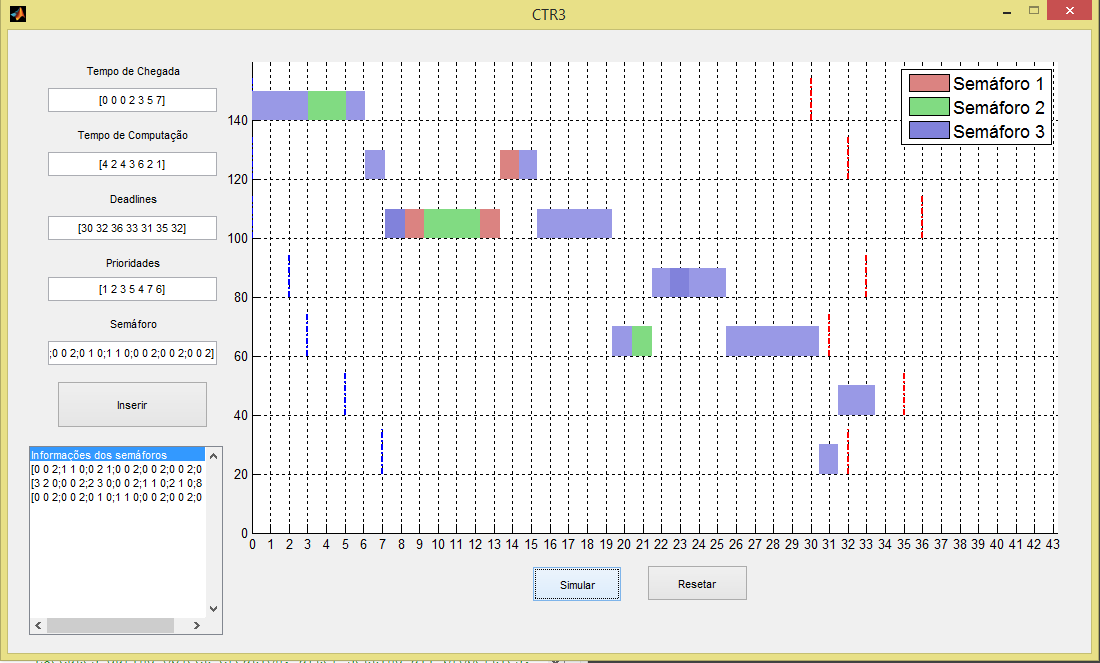
\includegraphics[keepaspectratio,width=1\textwidth]{img/teste1.png}
\end{figure}



\subsection{Teste 2}
\subsubsection{Configurações}
\begin{table}[H]
\centering
\caption{\em Tarefas.}
\vspace{0.1cm}
\begin{tabular}{c||c|c|c|c|c}
 
Parâmetros & $\tau_1$ & $\tau_2$ & $\tau_3$ & $\tau_4$ & $\tau_5$\\ 
\hline 
                          
$a_i$ & 0 & 0 & 3 & 5 & 7\\ 
$C_i$ & 4 & 2 & 6 & 3 & 2\\ 
$D_i$ & 6 & 11 & 20 & 30 & 25\\
$P_i$ & 1 & 2 & 4 & 6 & 5
 
\end{tabular}
\end{table}

\begin{table}[H]
\centering
\caption{\em Semáforo.}
\vspace{0.1cm}
\begin{tabular}{c||c|c|c||c|c|c}
 
Tarefas & $Sa_1$ & $Sa_C1$ & Status 1 & $Sa_2$ & $Sa_C2$ & Status 2\\ 
\hline 
                          
$\tau_1$ & 0 & 0 & 2 & 3 & 2 & 0 \\ 
$\tau_2$ & 1 & 1 & 0 & 0 & 0 & 2 \\
$\tau_3$ & 0 & 0 & 2 & 1 & 1 & 0 \\
$\tau_4$ & 0 & 0 & 2 & 2 & 1 & 0 \\
$\tau_5$ & 0 & 0 & 2 & 1 & 2 & 0 

\end{tabular}
\end{table}

\subsubsection{Resultado da Simulação}

\begin{figure}[H]
	\centering
	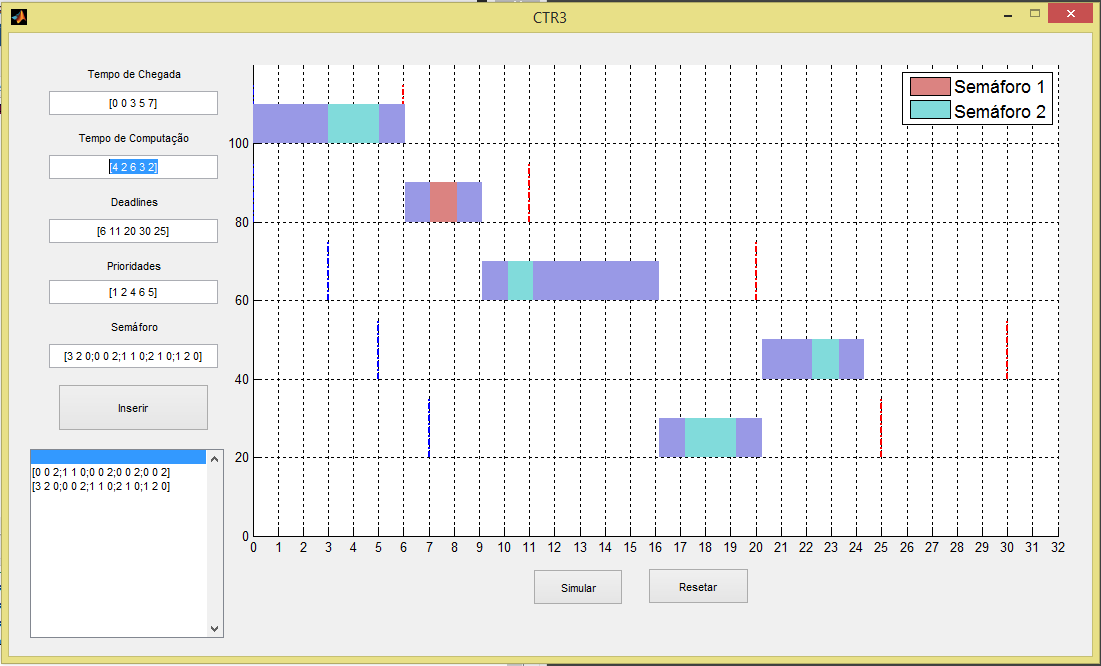
\includegraphics[keepaspectratio,width=1\textwidth]{img/teste2.png}
\end{figure}



\subsection{Teste 3}
\subsubsection{Configurações}
\begin{table}[H]
\centering
\caption{\em Tarefas.}
\vspace{0.1cm}
\begin{tabular}{c||c|c|c|c|c}
 
Parâmetros & $\tau_1$ & $\tau_2$ & $\tau_3$ & $\tau_4$ & $\tau_5$\\ 
\hline 
                          
$a_i$ & 0 & 0 & 3 & 5 & 7\\ 
$C_i$ & 4 & 2 & 6 & 3 & 3\\ 
$D_i$ & 6 & 13 & 20 & 29 & 25\\
$P_i$ & 1 & 2 & 4 & 6 & 5
 
\end{tabular}
\end{table}

\begin{table}[H]
\centering
\caption{\em Semáforo.}
\vspace{0.1cm}
\begin{tabular}{c||c|c|c}
 
Tarefas & $Sa_1$ & $Sa_C1$ & Status 1\\ 
\hline 
                          
$\tau_1$ & 3 & 2 & 0\\ 
$\tau_2$ & 1 & 4 & 0\\
$\tau_3$ & 1 & 1 & 0\\
$\tau_4$ & 2 & 1 & 0\\
$\tau_5$ & 1 & 2 & 0
 
\end{tabular}
\end{table}

\subsubsection{Resultado da Simulação}

\begin{figure}[H]
	\centering
	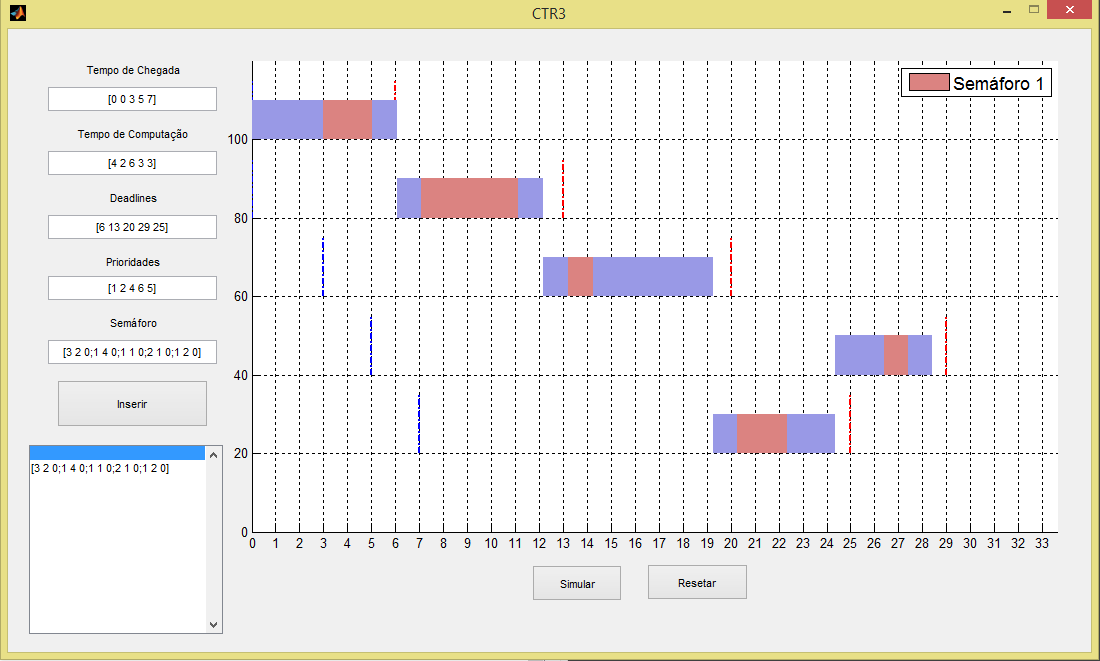
\includegraphics[keepaspectratio,width=1\textwidth]{img/teste3.png}
\end{figure}



\subsection{Teste 4}
\subsubsection{Configurações}
\begin{table}[H]
\centering
\caption{\em Tarefas.}
\vspace{0.1cm}
\begin{tabular}{c||c|c|c|c|c|c|c|c}
 
Parâmetros & $\tau_1$ & $\tau_2$ & $\tau_3$ & $\tau_4$ & $\tau_5$ & $\tau_6$ & $\tau_7$ & $\tau_8$\\ 
\hline 
                          
$a_i$ & 1 & 0 & 0 & 0 & 0 & 0 & 0 & 0\\ 
$C_i$ & 4 & 2 & 7 & 5 & 6 & 3 & 3 & 9\\ 
$D_i$ & 30 & 32 & 36 & 33 & 37 & 43 & 45 & 55\\
$P_i$ & 1 & 2 & 3 & 5 & 4 & 7 & 6 & 8
 
\end{tabular}
\end{table}


\begin{table}[H]
\centering
\caption{\em Semáforos 1.}
\vspace{0.1cm}
\begin{tabular}{c||c|c|c||c|c|c}
 
Tarefas & $Sa_1$ & $Sa_C1$ & Status 1 & $Sa_2$ & $Sa_C2$ & Status 2\\ 
\hline 
                          
$\tau_1$ & 0 & 0 & 2 & 3 & 2 & 0\\ 
$\tau_2$ & 1 & 1 & 0 & 0 & 0 & 2\\
$\tau_3$ & 0 & 2 & 1 & 2 & 3 & 0\\
$\tau_4$ & 0 & 0 & 2 & 0 & 0 & 2\\
$\tau_5$ & 0 & 0 & 2 & 1 & 1 & 0\\
$\tau_6$ & 0 & 0 & 2 & 2 & 1 & 0\\
$\tau_7$ & 0 & 0 & 2 & 1 & 2 & 0\\
$\tau_8$ & 0 & 0 & 2 & 0 & 0 & 2

\end{tabular}
\end{table}


\begin{table}[H]
\centering
\caption{\em Semáforos 2.}
\vspace{0.1cm}
\begin{tabular}{c||c|c|c||c|c|c}
 
Tarefas & $Sa_3$ & $Sa_C3$ & Status 3 & $Sa_4$ & $Sa_C4$ & Status 4\\ 
\hline 
                          
$\tau_1$ & 0 & 0 & 2 & 0 & 0 & 2\\ 
$\tau_2$ & 0 & 0 & 2 & 0 & 0 & 2\\
$\tau_3$ & 0 & 1 & 0 & 0 & 0 & 2\\
$\tau_4$ & 1 & 1 & 0 & 0 & 0 & 2\\
$\tau_5$ & 0 & 0 & 2 & 0 & 0 & 2\\
$\tau_6$ & 0 & 0 & 2 & 0 & 0 & 2\\
$\tau_7$ & 0 & 0 & 2 & 0 & 0 & 2\\
$\tau_8$ & 0 & 0 & 2 & 3 & 1 & 0

\end{tabular}
\end{table}

\subsubsection{Resultado da Simulação}

\begin{figure}[H]
	\centering
	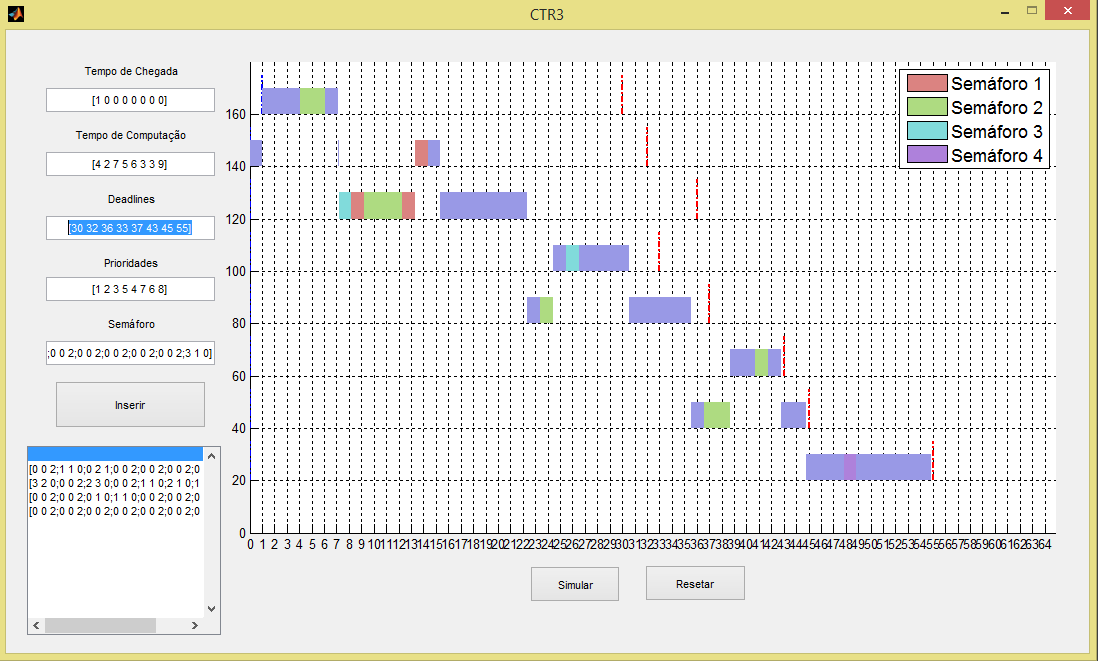
\includegraphics[keepaspectratio,width=1\textwidth]{img/teste4.png}
\end{figure}
\section{Anexo}

\end{document}